%%%%%%%%%%%%%%%%%%%%%%%%%%%%%%%%%%%%%%%%%%%%%%%%%%%%%%%%%%%%%%%%%%%%%%%%%%%%%%%
%%                                                                           %%
%%   Dr Varun Ojha                                                           %%
%%   Lecturer, Department of Computer Science                                %% 
%%   University of Reading, UK                                               %%
%%                                                                           %%
%%%%%%%%%%%%%%%%%%%%%%%%%%%%%%%%%%%%%%%%%%%%%%%%%%%%%%%%%%%%%%%%%%%%%%%%%%%%%%%
%%%%     SETTING STARTS - DO NOT CHANGE Unless your Tex setting require so   %%
%%%%%%%%%%%%%%%%%%%%%%%%%%%%%%%%%%%%%%%%%%%%%%%%%%%%%%%%%%%%%%%%%%%%%%%%%%%%%%%
%%----------------------------------------------------------------------------------
% DO NOT Change this is the required setting A4 page, 11pt, onside print, book style
%%----------------------------------------------------------------------------------
\documentclass[a4paper,11pt,oneside]{book} 

%%-------------------------------------
%% Page margin settings - % half inch margin all sides (recommended)
%%-------------------------------------
\usepackage[margin=1.2in]{geometry} 

%%-------------------------------------
%% Font settings - % CM San or Arial (recommended)
%%-------------------------------------
% Switch the following two line off: to revert back to defult LaTex font (NOT recomended)
\usepackage{amsfonts}
\renewcommand*\familydefault{\sfdefault}

%%-------------------------------------
%% Math/Defination/Theorem/Algorithm packages settings 
%%-------------------------------------
\usepackage[cmex10]{amsmath}
\usepackage{amssymb}
\usepackage{amsthm}
\newtheorem{mydef}{Definition}
\newtheorem{mytherm}{Theorem}

%%-------------------------------------
%% Algorithms/Code Listing environment settings  - 
%% Please do not change these settings
%%-------------------------------------

\usepackage{pythonhighlight}

\usepackage{algorithm}
\usepackage{algpseudocode}
\renewcommand{\algorithmicrequire}{\textbf{Input:}}
\renewcommand{\algorithmicensure}{\textbf{Output:}}
\usepackage[utf8]{inputenc}
\usepackage{listings}
\usepackage{xcolor}
\definecolor{codegreen}{rgb}{0,0.6,0.1}
\definecolor{codegray}{rgb}{0.5,0.5,0.5}
\definecolor{codeblue}{rgb}{0.10,0.00,1.00}
\definecolor{codepurple}{rgb}{0.58,0,0.82}
\definecolor{backcolour}{rgb}{1.0,1.0,1.0}
\lstdefinestyle{mystyle}{
    backgroundcolor=\color{backcolour},   
    commentstyle=\color{codegreen},
    keywordstyle=\color{codeblue},
    numberstyle=\tiny\color{codegray},
    stringstyle=\color{codepurple},
    basicstyle=\ttfamily\footnotesize,
    breakatwhitespace=false,         
    breaklines=true,                 
    captionpos=b,                        
    keepspaces=true,                 
    numbers=left,                    
    numbersep=5pt,                  
    showspaces=false,                
    showstringspaces=false,
    showtabs=false,                  
    tabsize=2,
    frame=none
}
\lstset{style=mystyle}

%%-------------------------------------
%% Graphics/Figures environment settings
%%-------------------------------------
\usepackage{graphicx}
\usepackage{subfigure}
\usepackage{caption}
\usepackage{lipsum}

%%-------------------------------------
%% Table environment settings
%%-------------------------------------
\usepackage{multirow}
\usepackage{rotating}
\usepackage{makecell}
\usepackage{booktabs}
%\usepackage{longtable,booktabs}

%%-------------------------------------
%% List of Abbreviations settings
%%-------------------------------------
\usepackage{enumitem}
\newlist{abbrv}{itemize}{1}
\setlist[abbrv,1]{label=,labelwidth=1in,align=parleft,itemsep=0.1\baselineskip,leftmargin=!}

%%-------------------------------------
%% bibliography/Refernces settings   - Harvard Style was used in this report
%%-------------------------------------
\usepackage[hidelinks]{hyperref}
\usepackage[comma,authoryear]{natbib}
\renewcommand{\bibname}{References} % DO NOT remove or switch of 

%%-------------------------------------
%% Appendix settings     
%%-------------------------------------
\usepackage[toc]{appendix}
%%%%%%%%%%%%%%%%%%%%%%%%%%%%%
%%%%     SETTING ENDS  %%%%%%
%%%%%%%%%%%%%%%%%%%%%%%%%%%%%
\begin{document}

    \captionsetup[figure]{margin=1.5cm,font=small,name={Figure},labelsep=colon}
    \captionsetup[table]{margin=1.5cm,font=small,name={Table},labelsep=colon}
    \setlipsumdefault{1}
    
    \frontmatter
          
    \begin{titlepage}      
        \begin{center}
            
\includegraphics[width=3cm]{figures/uorlogo.png}\\[0.5cm]
            {\LARGE University of Reading\\[0.5cm]
                Department of Computer Science}\\[2cm]
            %{\color{blue} \rule{\textwidth}{1pt}}
            
            % -------------------------------
            % You need to edit some details here
            % -------------------------------  
            
            %------------------------------  TITLE of Your PROJECT ----------------------------------%
            % chnage the following line
            \linespread{1.2}\huge {Predicting booking cancellations using machine learning}
            
            
            \linespread{1}~\\[2cm]
            %{\color{blue} \rule{\textwidth}{1pt}}
            
            %------------------------------  Your Name  -------------------------------%
            % chnage the following line
            {\Large Samuel Pink}\\[1cm] 
            
            %-------------------------- Your Superviosr's name(s) ---------------------%
            % chnage the following line
            {\large \emph{Supervisor:} Bryan Lawrence}\\[1cm] % if applicable
            
            % PLEASE DO NOT CHANGE THIS TEXT %
            \large A report submitted in partial fulfilment of the requirements of\\the University of Reading for the degree of\\ Bachelor of Science in \textit{Computer Science}\\[0.3cm] 
            \vfill
            
            
            \today % Please update this date you can use \date{April 2020} for fixed date
        \end{center}
    \end{titlepage}

    % -------------------------------------------------------------------
    % Declaration
    % -------------------------------------------------------------------
    \newpage
    \thispagestyle{empty}
    \chapter*{\Large Declaration}
    % PLEASE CHANGE THIS TEXT EXCEPT YOUR NAME%
    % -------------------------------
    % PLEASE ONLY UPDATE HERE -- PLEASE WRITE YOUR NAME %    
    % ------------------------------- 
    I, Samuel Pink, of the Department of Computer Science, University of Reading, confirm that all the sentences, figures, tables, equations, code snippets, artworks, and illustrations in this report are original and have not been taken from any other person's work, except where the works of others have been explicitly acknowledged, quoted, and referenced. I understand that if failing to do so will be considered a case of plagiarism. Plagiarism is a form of academic misconduct and will be penalised accordingly.\\[1cm]
    
    
    \begin{flushright}
        %------------------------------ PLEASE UPDATE  Your Name  -------------------------------%
        % change the following line
        Samuel Pink % Please change it to your name
        
        \today
    \end{flushright}
     
    % -------------------------------------------------------------------
    % Abstract and Acknowledgement
    % -------------------------------------------------------------------
    
    \chapter*{\center \Large  Abstract}
..

~\\[1cm]
\noindent
\textbf{Keywords:} ...

\vfill
\noindent
\textbf{Report's total word count:} ...


    % -------------------------------------------------------------------
	% Acknowledgement
	% -------------------------------------------------------------------
   
    %\chapter*{\center \Large  Acknowledgments}

Acknowledgments section is optional. You may like to acknowledge the support and help of your supervisor(s), friend(s), or any other person(s), department(s), institute(s).

   
    
    % -------------------------------------------------------------------
    % Contents, list of figures, list of tables
    % -------------------------------------------------------------------
    
    \tableofcontents
    %\listoffigures
    %\listoftables
    
    % -------------------------------------------------------------------
    % Main chapters and sections of your Project
    % Everything from here on your words and works 
    % -------------------------------------------------------------------
    \mainmatter
    % Read for preparation of document in LaTex 
    % Lamport, L. (1986), LATEX: A Document Preparation System, Addison-Wesley.
    
    \chapter{Introduction}

Machine learning will be used to analyse student accommodation bookings with a focus on the ability to reliably estimate revenue in order to determine when a contract will not be fulfilled. This will be completed utilising data from the property management system \cite{Jain2006IntellectualPerspective}.

\section{Background}

A contract made in advanced between the student (customer) and the company, defines the services that will be sold (the room), as well as the start and end date of the tenancy and the fixed price the service will be sold at. In the case of student accommodation, this contract is usually made a few months in advance, in some cases before the student has finalized their plan to attend a specific university. Because of this, the student withholds the right to cancel the contract before it is paid. The inherent uncertainty of the contract means there is no way for the company to definitively measure what the occupancy and sales of a given property will be in advance, since they have to take on the risk of cancellation. This problem is not unique to the student property sector; it is a revenue management issue that was first identified by the aviation industry in 1966 \cite{Chiang2007AnResearch}.

\vspace{5mm}

Having the ability to predict with some degree of certainty whether or not a booking is going to be cancelled would allow for more accurate decisions about revenue management to be made and overcome some of the risk created with a contract based booking system.When this is performed with machine learning, the accuracy of the predictions can improve over time as a result of a better understanding of the data, new iterations of modelling, and comparisons of the actual and predicted outcomes. In the case of booking management, a lot of data is stored about each booking made, so the ability of a machine learning algorithm to make accurate predictions on a given outcome is dependent on the data available to it, the amount of data, as well as the accuracy and usability of the data. This means that it should be possible with the correct classification techniques to make accurate predictions on the outcome of the booking.

\section{Problem Statement}

In total for the year 2020 to 2021, 25 percent of all 14363 bookings in the dataset were cancelled, accounting for over 20 million pounds in revenue loss from customers who completed the booking process and then cancelled before the contract was paid. There are a number of different reasons that account for each booking being cancelled that range from impact caused due to Coronavirus and students not receiving their target grades. In most of these cases, the student will then choose to stay at different accommodation resulting in the sale being lost. Producing a model that is able to predict which of these bookings will be cancelled in real time would then allow the business to take actions to try and prevent the student from cancelling their booking. Being able to prevent just 10 percent of users from cancelling would therefore create a potential gain of 2 million in revenue per year.  

\vspace{5mm}

On a small scale, recognising the characteristics that are common among cancelled bookings would be relatively simple; for example, looking at the percentage of cancelled bookings in the previous year, an approximate estimate of the number of bookings that would be cancelled this year could be estimated. Then, to figure out why these bookings were cancelled, look at what these bookings have in common. In this case, however, no amount of human analysis could possibly account for all of the factors, given that the organisation operates over 70,000 beds worldwide. The fact that a student has the right to cancel a reservation up until a certain time period for a specified penalty means that it is the provider's duty to account for the inherent ambiguity of the contract . The most common method to solve this problem is to simply take the number of bookings cancelled in the previous year and use that number as an average to measure the number of bookings expected to be cancelled in the current year. The problem with this approach is that it only considers one of the many factors, previous year figures, while the company actually keeps hundreds of data points for each booking. Therefore, this problem is going to be attempted to be solved using  machine learning. Since the dataset used comes directly from the company in question and includes actual data about students, all personal information has been removed. Instead, students and properties will be referred to solely by their IDs, ensuring that both the company and the students remain anonymous.
    
\section{Aims and objectives}

By combining all relevant data points from previous years' bookings, a model that can classify a booking into two distinct states, cancelled or not cancelled, is going to be created. It's important to not only build a model that predicts which bookings will be cancelled, but also to understand why bookings are cancelled by using the model to determine which features in the dataset have the greatest impact on whether or not a customer will cancel. This is critical in assisting the company to make business decisions based on the data in order to not only avoid the cancellation but also to understand what actions can be taken to reduce the number of cancellations in the future.

\vspace{5mm}

The first step in solving any machine learning problem is obtaining accurate and clean data. In most cases (including this one), this is the most difficult problem to solve because data is rarely stored in a way that makes it easy to read and analyse; in fact, data is frequently stored and then never used. To rectify this, first of all a data warehouse will be created in which to store and analyse the data and then creating a classification model \cite{SessionsTHEALGORITHMS}. This data warehouse will exist in the Azure cloud on top of Docker Containers with the code written in Python, with the aim being to create a stream to import new booking data into the data warehouse hourly ensuring that it is stored in a way that makes it easy to use for model training. The aim is to integrate the classification model into the booking management system by creating a daily list of which customers are most likely to cancel their bookings to the managers of their respective properties along with the recommended actions to be taken to prevent the cancellation. Storing the data of the actions taken and whether or not it was successful can then be used to improve future iterations of the model.

\section{Solution approach}

To create a classification model on the booking dataset, the AutoML feature of Azure ML Studio will be used. Auto ML is used because it automates the process of cross validations and feature engineering, which significantly speeds up the model development process. AutoML is able to take advantage of the cloud resources made available through the company by running multiple models at the same time and increasing the speed with which individual models are executed. Bookings will be classified into two distinct groups: cancelled or not cancelled. This is a binary classification because there are only two states in which a booking can be classified. There are two types of classification approaches: supervised and unsupervised learning. This is an example of supervised learning because the expected values are known. Machine learning's aim is to take a set of data with predefined outputs and construct a function that maps the relationship between the inputs and outputs.

 \begin{figure}[H]
 \centering
 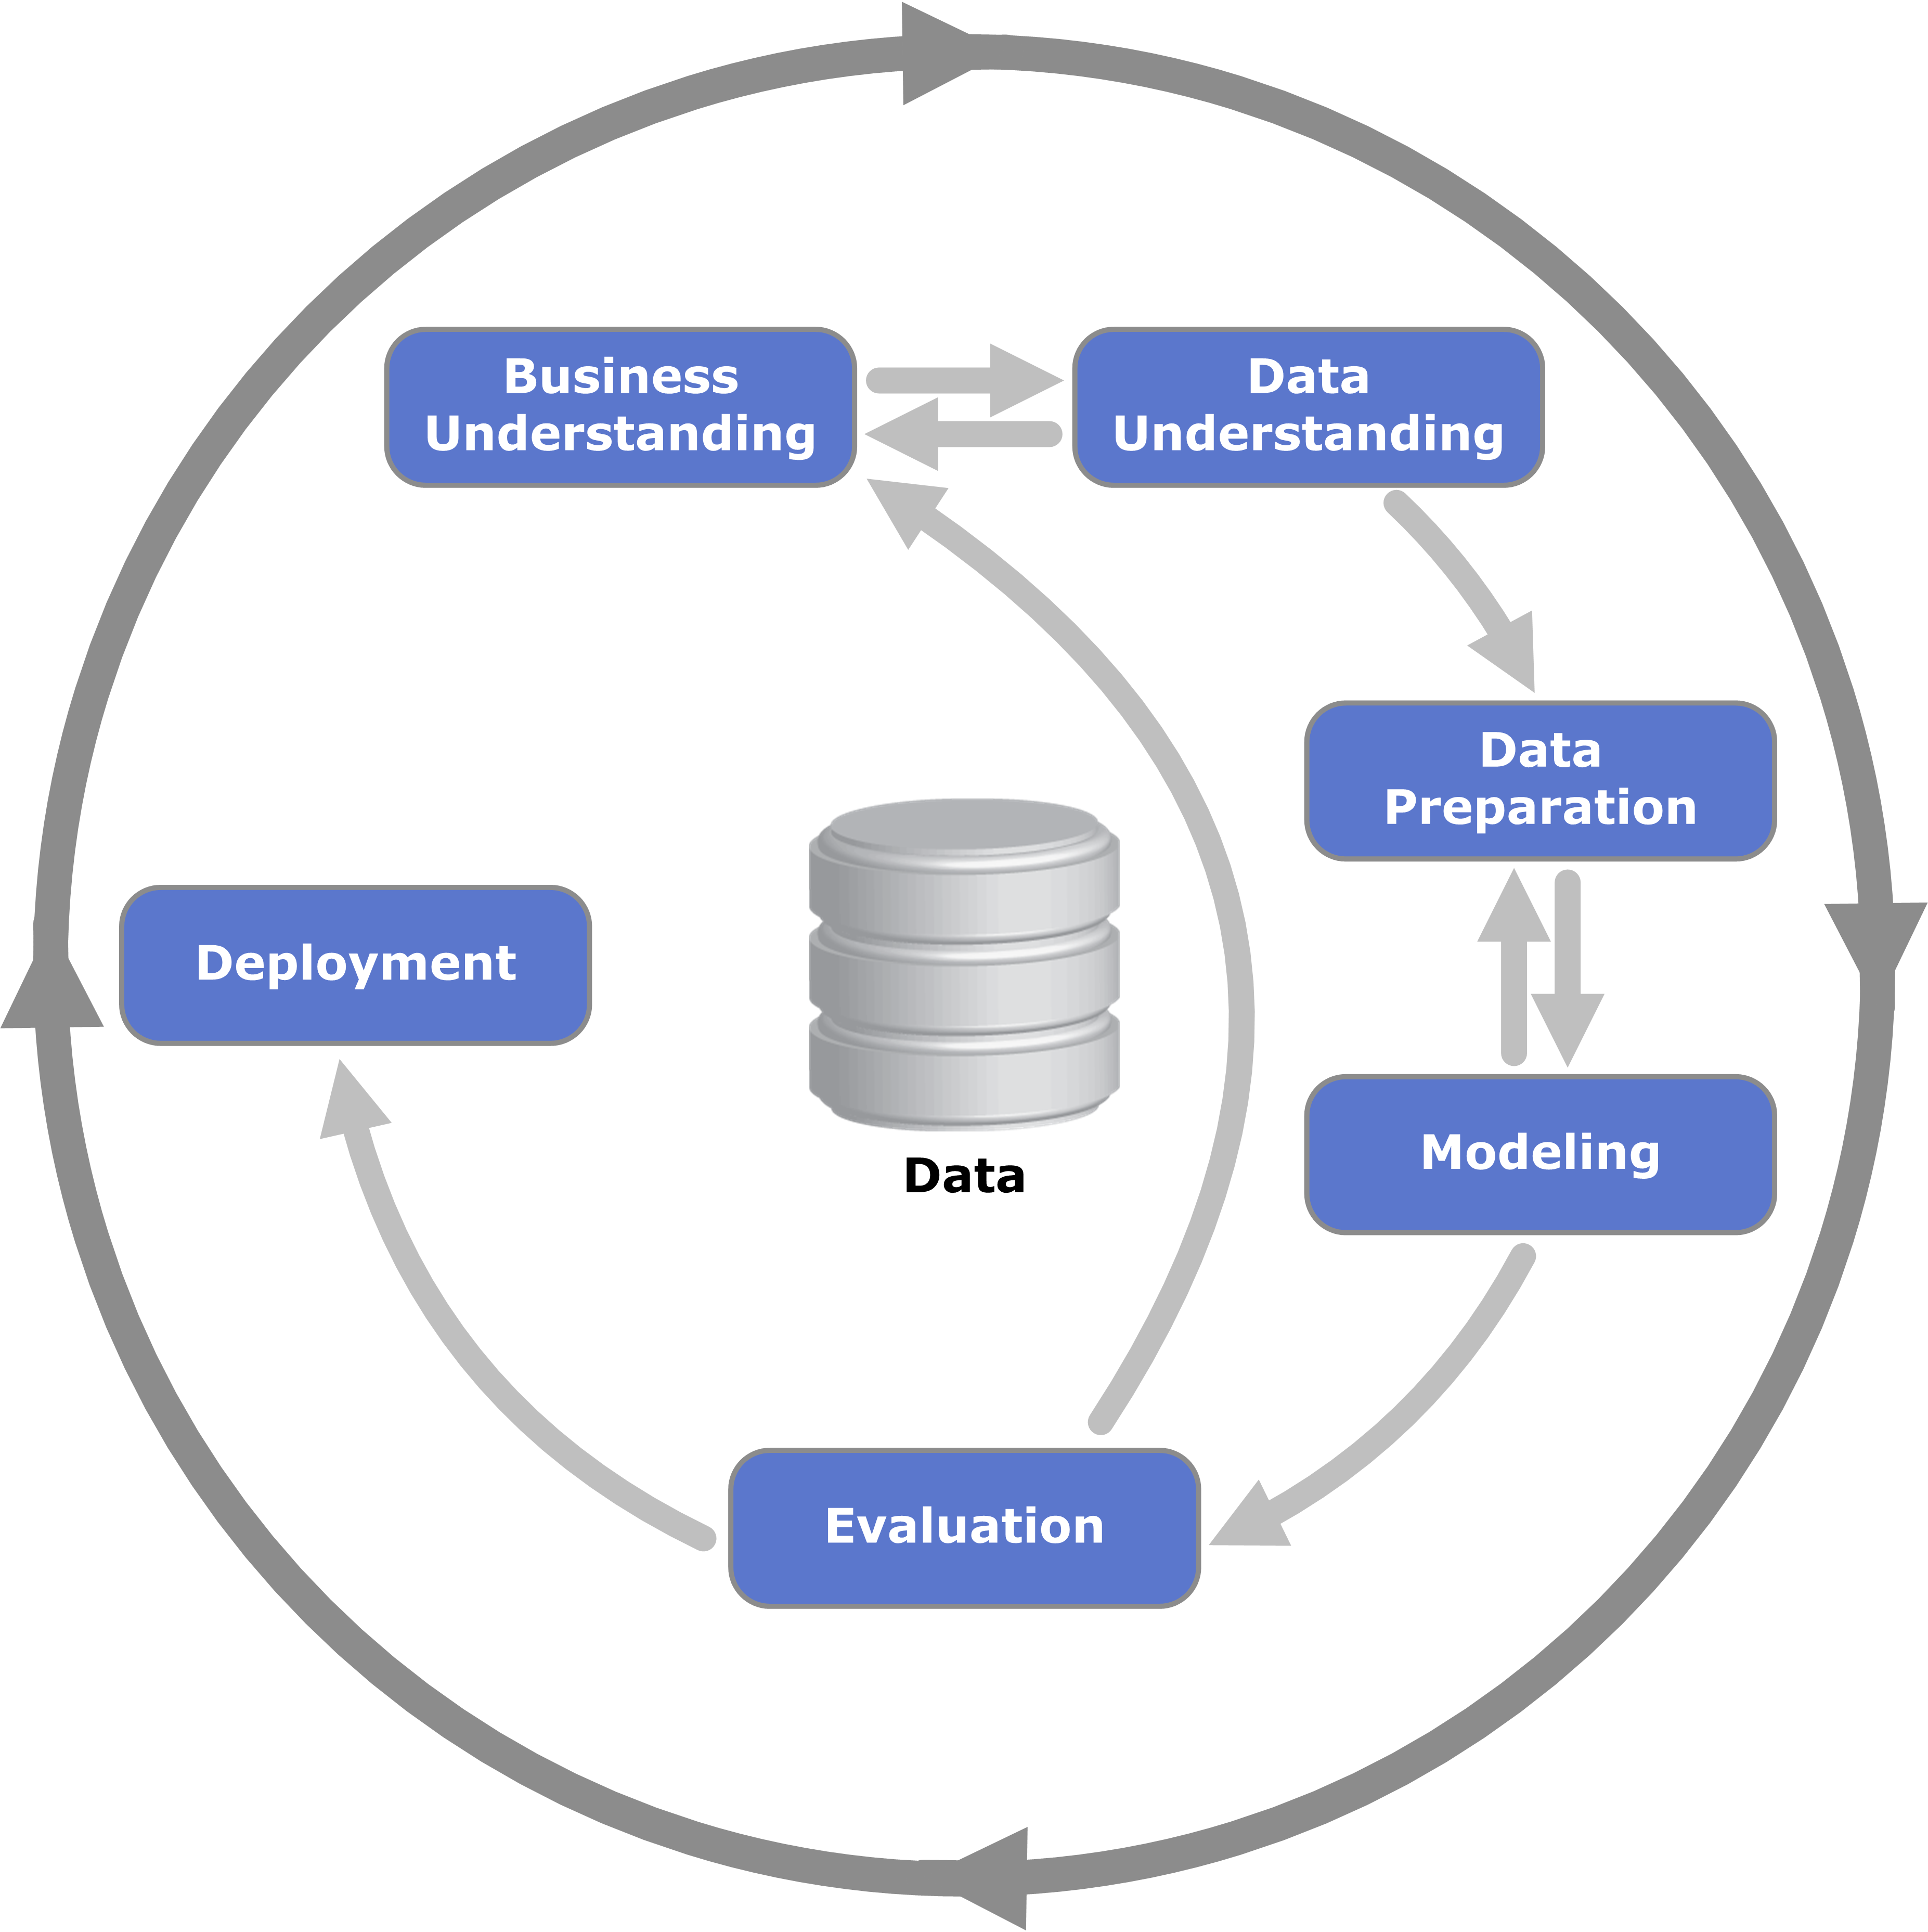
\includegraphics[width=10cm]{figures/CRISPDM_Process_Diagram.png}
 \caption{The six stages of the CRISP-DM process identified are used to break down the methodology. This diagram depicts the relationship between the various phases of CRISP-DM, demonstrating the sequential design of a data mining project.}
\end{figure} 


The most popular data-mining model is the Cross Industry Standard Method for Data Mining (CRISP-DM), according to current research, due to its numerous advantages, which solved existing data-mining problems \cite{Wirth2000CRISP-DMMining}. It works by breaking the problem down into six stages, as shown in Figure 1.1: business understanding, data understanding, data preparation, modelling, evaluation, and deployment.

\vspace{5mm}

To determine the best approach to solving the problem,  first the company employees were consulted to gain a better understanding of the types of results that would be most effective, as well as the actions that can be taken to have the best chance of preventing a cancellation at the individual booking level. It was discovered that it is critical the results can be presented in a way that employees can understand so that appropriate actions can be taken. Creating a table that ranked bookings by highest probability of cancellation was also discovered to be the best way to display the model's results. Another feature that was found to be important is the ability to retrain the model on new data and adjust the hyper tuning parameters, because the booking dataset is constantly being updated with new entries and it is constantly evolving.

\vspace{5mm}

One of the problems that needed to be solved was how to get access to data that is suitable for machine learning, the data preparation stage. This stage consistently requires the most time as seen in previous literature \cite{Zhang2003DataMining}. To perform machine learning, data needs to be accessible in a suitable format and stored appropriately. The current booking system behind the dataset in this research does not store the data in a way that is suitable for use in machine learning. Building a data warehouse allows for the data to be converted into an appropriate format for machine learning problems. The ability of the data warehouse to update upon new bookings and provide instant access to the data, a feature of the data warehouse using Azure cloud that was used in this project, is an important aspect. The main technology used throughout the modeling process will be Auto ML studio as a framework to encapsulate all of the tools needed to complete a machine learning project, it allows for direct connection to the database for accessing the data through integrated Jupiter Notebooks. Use of Jupiter Notebooks in Python provides an environment for the data cleaning and preparation stages that need to be performed entirely within the azure cloud. The modeling stages are done in the same way by importing the Auto ML Python SDK into the Jupiter Notebook. The Experiment class (azureml.core.experiment.Experiment) in the SDK is used to store and run the models within a logical resource group with the ability to add and remove different modeling iterations from the experiment as well as viewing the results. When a model is configured through AutoMLConfig (azureml.train.automl.automlconfig.AutoMLConfig), it is then added to the experiment and the run is executed in the cloud. Undertaking this process in the cloud helps to solve the General Data Protection Regulation (GDPR) related problems of data access as the data is never stored on the local computer.


\vspace{5mm}

The intended outcome of this research is to have the ability to rank bookings by the probability of them being cancelled, providing a platform to integrate the model's results into the company's booking system. Doing this would allow the company to have the ability to input whether or not the prediction was correct. The model would then be able to be retrained based on the outcomes of the predictions, over time allowing for the models accuracy to be increased. 
    \chapter{Literature Review}
\label{ch:lit_rev}

\section{Business Perspective}

Revenue management is defined as “the application of information systems and pricing strategies to allocate the right capacity to the right customer at the right price at the right time” \cite{Kimes2003HasAcceptable}. This is essential to a company selling a fixed number of rooms, setting the price too high would result in customers moving to competitors and cause reduced profits as well as a poor customer experience. Setting the price too low however may result in maximum occupancy but will trade this for potential losses in overall profits.

\vspace{5mm}

Booking cancellations are one of the main focuses in the revenue management industry as a whole \cite{Subramanian1999AirlineNo-shows}. Since a trade-off needs to be made between implementing a ridged cancellation policy that imposes penalties on cancellation, and a policy that has no impact to the customer. \cite{Jinhong2007ServiceCancellations} shows that implementing a rigid cancellation policy can act as a sales inhibitor and therefore reduce the number of customers. This however further increases the uncertainty as there is little impact to customers cancelling bookings. \cite{Talluri2004TheManagement} finds that in some cases customers looking for the best price will make multiple bookings and then cancel all but one. 

\vspace{5mm}

Looking at this problem specifically in the student accommodation industry, more focus needs to be directed towards capacity and price, this is unlike the hotel industry which deals more with short term stays. In the student accommodation data used for this research the mean stay is 247 days and once the room is sold it is set at this fixed price for the duration of the academic year.

 \vspace{5mm}
 
Demand forecasting is one of five revenue management issues; the others are pricing, auctions, capacity management, and overbooking. The development of a booking cancellation prediction model follows \cite{Chiang2007AnResearch} recommendation that sales management should use statistical and projection models to best use available data and technologies.
 
\vspace{5mm}

As mentioned by \cite{RevenueWorldCat.org} and \cite{Weatherford2003AManagement}, having the ability to accurately forecast demand is key to revenue management in determining how many rooms will be sold and to calculate the correct price at which to sell rooms. This ability to forecast demand then needs to be used in creating the correct pricing model "in which a perishable and nonrenewable set of resources satisfy stochastic price sensitive demand processes over a finite period of time" \cite{Bitran2003AnManagement}.

\vspace{5mm}

Using what was identified by \cite{Talluri2004TheManagement} that “science and technology now make it possible to manage demand on a scale and complexity that would be unthinkable through manual means”; this study aims to use the tools now available in the field of machine learning and the increased number of data points on each customer to approach the prediction of cancellations as a classification problem. This backs up "Demand-based pricing is underused in many service industries" \cite{Kimes2003HasAcceptable} implying that a limited number of industries have properly taken advantage of new technology available in the field of machine learning.

\vspace{5mm}

\cite{Newell2018TheSector} stated "Amongst the alternative property sectors, student accommodation has recently become an important institutionalised property sector". In the UK alone the student accommodation industry is worth around 60 Billion \cite{UKWakefield} with an increase of 14 percent over the last 5 years \cite{UKWakefield}. Despite this, there is no research in the field of forecasting or analysing demand. With the recent impact of COVID-19 causing a large number of students to have to study from home and in some cases no longer needing student accommodation it is more important than ever to have the ability to accurately forecast the demand. 

\section{Choice of algorithm}

Machine Learning algorithms use statistics to find correlations for large quantities of data, if data can be processed in digital form and fed into a machine learning algorithm.\cite{Chen2019MehryarEdition}. Machine learning algorithms make use of data to increase accuracy and to simulate accurately. Teaching a system can be much simpler than manually programming by showing samples of desired input behaviour in anticipation of the requested answer with all potential inputs.\cite{Jordan2015MachineProspects}. 

\vspace{5mm}

Using machine learning to forecast bookings can be separated into two specific types of problems, regression problems where the aim is to predict a continuous quantitative value like the sum of bookings that will be cancelled in a given year, and classification where each booking can be classified into two groups: cancelled or not cancelled. Most of the research in this field is focused on solving it as a regression problem with  \cite{RomeroMorales2010ForecastingMining} stating “it is hard to imagine that one can predict whether a booking will be cancelled or not with high accuracy simply by looking at Passenger Name Record (PNR) information”. PNR data does not store the same number of data points as property management system data, it is a file containing information about a passenger (or a travelling group) and their travel plans in the system's database.

\vspace{5mm}

XGBoost is a distributed gradient boosting library that has been optimised for performance, flexibility, and portability \cite{Chen2016XGBoost:System}. It uses the Gradient Boosting framework to implement machine learning algorithms. XGBoost is a parallel tree boosting algorithm that solves a variety of data science problems quickly and accurately. XGBoost is commonly used by data scientists to produce cutting-edge performance on a variety of machine learning problems. Various interfaces are supported by XGBoost, including the Python interface. The implementation of XGBoost focuses on computational speed, model performance and memory resources.The most critical element in XGBoost's performance is its scalability in all situations. On a single machine, the device is more than ten times faster than current common solutions, and it scales to billions of examples in distributed or memory-limited environments \cite{ChenXGBoost:System}.

\vspace{5mm}

At its most basic level, decision tree analysis is a strategy for classification that can be used to identify and remove important features and patterns from databases to allow for discrimination and modelling predictions. These characteristics, combined with their intuitive interpretation, explain why decision trees have been widely used for over two decades in exploratory data analysis and predictive modelling applications \cite{Myles2004AnModeling}. Due to its efficiency, accuracy, and interpretability, gradient boosting decision trees (GBDT) are a widely used machine learning algorithm. GBDT outperforms the competition in a variety of machine learning tasks. With the advent of big data in recent years, GBDT has encountered new challenges, most notably in the accuracy-efficiency trade-off \cite{KeLightGBM:Tree}.

\section{Summary}

Current research focuses on looking at prediction cancellations mainly in the hotel and aviation industry, expanding this use of machine learning on revenue management into the student accommodation industry provides more knowledge on how machine learning can be applied to other industries. 


% https://guides.library.bloomu.edu/litreview
    \chapter{Methodology}
\label{ch:method}
...

\section{...}
To account for the multiple different stages involved in the Data Mining process I am going to be using the CRISP-DM process (\cite{WirthCRISP-DM:Mining}) to break down the problem into 6 specific stages


\section{Business Understanding}

The booking data relevant to this problem is stored in an external system, this is the website front facing to the customers where each of the bookings are taken. As a booking is made through the website customer details are stored in the databases this data includes personal information of the customer like name, address, date of birth and phone number. As the customer moves further through the booking process they are then taken to a page asking which university they will be attending and to make a selection of the property they want to rent, here information like location of property, room name, price and extras as stored. when a student then selects a specific room they will be asked about the payment structure they want to use and how they will make there deposit. it is here that all of the relevant cost data is stored. \par

The information stored within these stages of the booking describes all of the intellectual property stored about each specific customer and therefore is what will be used to predict the activity of the customer and weather or not they will cancel there booking. 

In total the dataset contains 45 properties in 5 countries with a large variation in price depending on city and room selection 


\section{Data Understanding}
\textbf{
\begin{itemize}
\item include the total size of each property 
\item include lead time
\end{itemize}
}

In the case of a classification problem we can consider any attribute relevant if it influences the target variable. With the common goal in machine learning to obtain as much useful information as possible since [reference good number of data points for machine learning]

In this case I will be looking only at data from this year since the old data is shit. During this booking cycle there are a total of around 16 thousand bookings  in some number of countries 

Do I start with all and run analysis to find what is dependant 
Or start with a small set and only add things that seem important

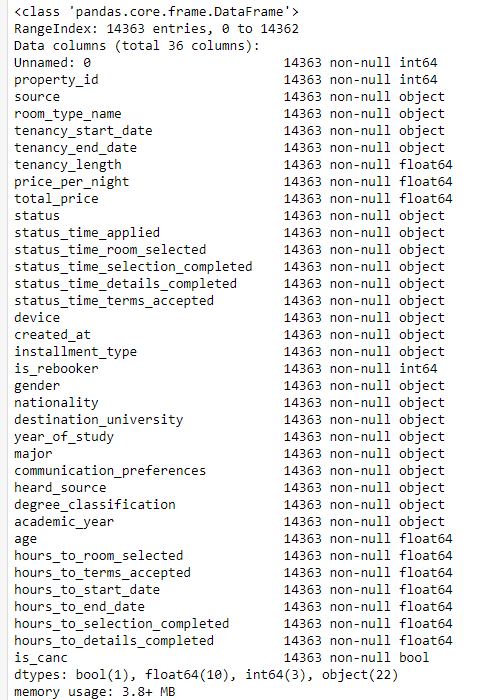
\includegraphics[width=10cm]{figures/df_info.png}


\begin{itemize}
    \item property id is the unique identifier for the residence 
    \item source is the internal system used to create the booking
    \item room type name is the category of room selected
    \item tenancy start date is the proposed start date of the contract
    \item tenancy end date is the proposed end date of the contract
    \item tenancy length is the duration in day the contract is valid for
    \item price per night is the daily rate at which the room will be sold
    \item total price is the total price for the contracted time
    \item status is the current status of the booking
    \item status time applied is the time the booking process was started
    \item status time room selected is the time the customer selected there room
    \item status time selection completed is the time the customer finalised the selected process 
    \item status time details completed is the time all personal details are entered
    \item status time terms accepted is the time the agreement is completed
    \item device is the type of the device the booking was made on
    \item created as is the time the process was started
    \item installment type is the payment schedule
    \item is rebooker defines if the same customer has applied before
    \item date of birth of the customer
    \item gender of the customer
    \item nationality of the customer
    \item destination university is the university the customer expects to go to
    \item year of study is the academic year  the customer is in
    \item major is the degree type of the student
    \item communication preference is the customer selected method of communication
    \item heard source is where the customer discovered the booking
    \item degree classification is the degree type of the customer
    \item academic year
 

\end{itemize}

 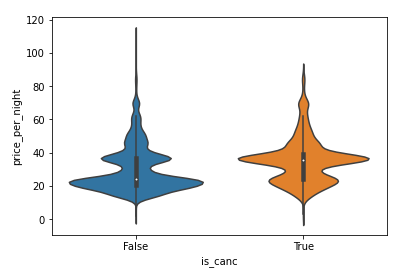
\includegraphics[width=10cm]{figures/price_per_night.png}
 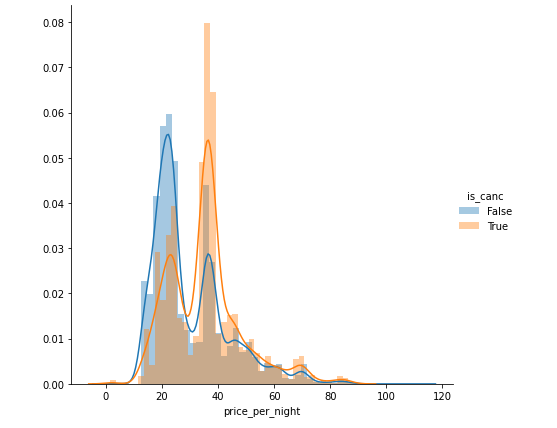
\includegraphics[width=10cm]{figures/price_per_night_2.png}
 
 looking at the price per night when comparing booking that canceled to ones that didn't we can see that around the middle price range of 40 euro per night is where the most significant number of bookings occur, the figure also shows more cancellations towards the higher end price points.  
 
 \textbf{how will this be used to help the model}
 
  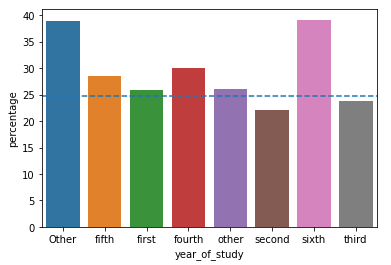
\includegraphics[width=10cm]{figures/canc_per_year.png}
  
  This figure shows a weighted proportion of customers canceling bookings in each year of study with the blue horizontal line being the average, we can see that sixth year students are more likely to cancel than any other year possibly because they are more likely to decide to live in private accommodation. the other category are students that didn't fill out the year of study section, this seems to be a good indication or cancellations.
  
  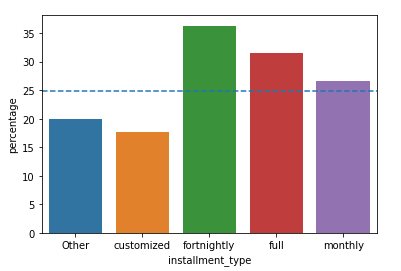
\includegraphics[width=10cm]{figures/instalment_type.png}
  
  This figure shows a weighted average of cancellations looking at the selected instalment type. instalment type is the payment plan the student selected, we can see that students who selected the fortnightly plan are 10 percent more likely to cancel than the average and students who opted for the customized installment plan are around 6 percent less likely to canceled. this many be a good predictor of cancellations.
  
  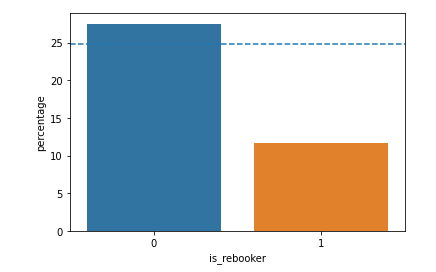
\includegraphics[width=10cm]{figures/is_rebooker.png}
  
  The figure above shows the comparison in cancellations with students who are rebookers (have booked before), we can see that students who have booked previously are around half as likely to cancel there bookings. this is another good predictor of cancellations.  
  

\section{Data Preparation}
\textbf{Do I include the data cleaning notebook here}

To get the relevant data for solving this problem I first had to approach the wider problem of developing a robust data warehouse [reference] I started by building a live and dynamic data stream that could take data from an external source and store it in the company data warehouse so I would be able to run new iterations of the model as new data came in. To facilitate the problem of having a dynamic data import stream I used the python object relation mapping library [\textbf{SQLAlchemy - The Database Toolkit for Python}] since it has direct support for the python data library pandas []. Doing this allows me to read data in any supported format [supported formats] and store it in a SQL database with the correct data types. the data I need is stored in an Amazon S3 bucket, so I used the python S3 library Boto3 to read TSV files from blob storage every hour and stored them in the data warehouse. I then deployed this process onto a docker container.

\vspace{5mm}

With all of the necessary data stored in the data warehouse I imported the relevant tables into a Jupiter Notebook to preform the data cleaning stages. My aim is to include only valid bookings that made it the whole way through the booking process and then separate into cancelled or not.

I started by removing any booking in the dataset that didn't have a total price or with a total price less than 1 as this meant the booking was not stored in the system correctly and may have been used for testing as this would affect the final model. 

I then removed any booking that did not get to the terms accepted stage since this could not be treated as a cancellation or a booking as the customer process was not finished.

Using the status time applied column to act as the first point where the booking process was started I created attributes used to store how long the customer took within each stage of the booking process as this may be able to indicate weather or not the user will cancel there booking.  \textbf{find a reference to support this}

\section{Modeling}

I used Azure ML Studio to evaluate and compare multiple diffident algorithms. 

I found that XGboost was the most accurate algorithm when comparing \textbf{some metrics}, because of this I chose to run the XGboost algorithm outside of the Azure ML environment to create a model that can be implemented more efficiently into the CHRISP-DM process

XGBoost is an optimized distributed gradient boosting library designed to be highly efficient, flexible and portable. It implements machine learning algorithms under the Gradient Boosting framework. XGBoost provides a parallel tree boosting (also known as GBDT, GBM) that solve many data science problems in a fast and accurate way. The same code runs on major distributed environment (Hadoop, SGE, MPI) and can solve problems beyond billions of examples. [XGBoost Documentation — XGBoost 1.4.0-SNAPSHOT documentation]

\begin{itemize}
\item splitting data into num and cat vars 
\item used SimpleImputer to replace missing num values with mean
\item train test split of 0.2
\end{itemize}

			 
Azure ml
Azure machine learning studio [What is Azure Machine Learning | Microsoft Docs] is a cloud environment that can be used to both train and deploy machine learning models 


\section{Evaluation}

\section{Deployment}



    \chapter{Results}
\label{ch:results}
\section{Comparing algorithms}



\begin{center}
\begin{tabular}{ c c}
 Model              & Accuracy \\
XGBoost            & 83\%     \\
LightGBM           & 82\%     \\
GradientBoosting   & 79\%     \\
LogisticRegression & 76\%   
\end{tabular}
\end{center}
\section{XGBoost}

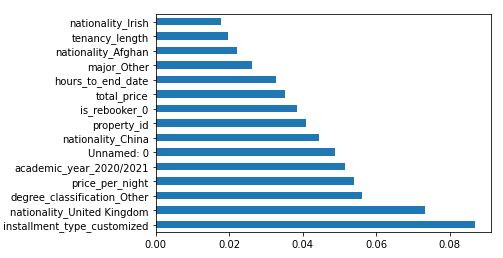
\includegraphics[width=10cm]{figures/results_features.png}

looking at the above figure we can see the feature with most influence on the Target variable is installment type, specifically instalment type customised. This is supported by figure [\textbf{something}] that show students with the instalment type customized are far less likely to cancel. The second most important feature of nationality United Kingdom is likely a dependant feature because the majority of bookings are made by students from the United Kingdom. 
\textbf{i think add a figure to methodology for nationality}
Degree type other being an influencing factor is also supported by figure [\textbf{something}] since students with degree type other where around twice as likely to cancel bookings.



\section{Using Azure ML}

\begin{figure}[hbt!]
 %\centering
 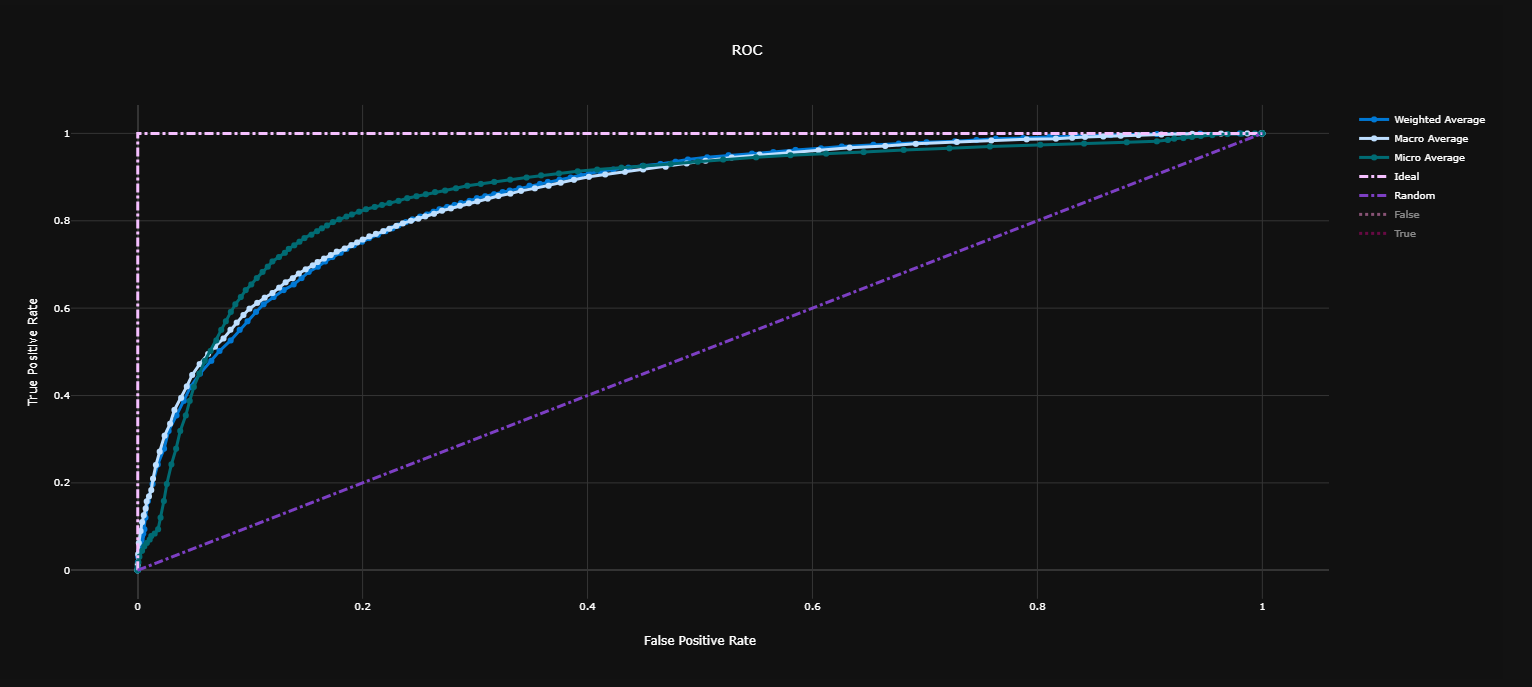
\includegraphics[width=10cm]{figures/azure_ml_roc.png}
 \caption{ROC curve (receiver operating characteristic curve) is a graph showing the performance of a classification model at all classification thresholds. This curve plots two parameters, false positive and true positive}
\end{figure}


    \chapter{Discussion and Analysis}
...

\section{..}
\begin{itemize}
\item In comparison to using the python libraries to create the models manually, using azure ml allowed for me to test a larger variety of algorithms and gaining more accurate results. Azure ml has built in functionality that allows for an explanation of the model and the results which can allow for a better understanding of the model results, such as the feature explanation. This subsequently can be used to retrain the model, further improving its accuracy. 
\item  From a machine learning point of view, using azure ml is beneficial to be able to test multiple different algorithms and select the one with the best results in a more efficient manner. This is also beneficial from the business perspective as it provides an explanation behind the results, allowing for insights into the models accuracy. From this specific dataset, Stack Ensemble was found to be the most accurate in predicting booking cancellations. Using azure ml allowed for Stack Ensemble to be identified as the best algorithm to be used on this dataset which would not have been identified otherwise. This has produced significantly better results in comparison to the original algorithm used, xgboost. 
\item The dataset used in this project was from the time period 2020-2021. There is a chance that the amount of cancellations and the reasons behind these could have been affected by the Coronavirus pandemic, potentially influencing the results of this model. In some cases students have been advised to stay at home and not live in halls during this time period, meaning that the booking would have been cancelled. This could have produced a dataset which is not fully representative of a normal academic year. However, the ratio of cancellations in this dataset was in line with previous research (\textbf{reference)}, suggesting that the pandemic may not have had an affect at all. There was no available data from before the Coronavirus pandemic which could be used in this project. In order to be sure that the dataset was not affected by the Coronavirus pandemic, these findings should be compared to future years.
\item However, there are some valuable insights that can be gained from this project regardless of Coronavirus. It is likely that the Coronavirus pandemic will still have a significant impact on the student accommodation industry in the next academic year. Being able to analyse the 2020-2021 booking data has allowed for the prediction of cancellations and the reasons behind these. This can be useful to determine business strategies to implement with the aim to reduce student accommodation cancellations in the next academic year. 
\item Due to insufficient amount of data for some properties, the model in this project used all properties to predict cancellations. It is likely that creating a model that predicts cancellations on a per property basis would be more accurate. This is reinforced by previous research in revenue management which uses a per property level for there models \textbf{(reference)}. A per property model would likely be more accurate as each property has different attributes and different potential reasons for cancellations. For example, the properties in this dataset were in a variety of countries, at different universities and the price varied heavily depending on location. Although the findings of this model were still useful, future research should focus on using more data and making the model property specific. 
\item \textbf{how results compare with similar papers in revenue management }
\item As with all machine learning problems, the model is most accurate when trained over a number of iterations. This usually takes a long time in writing the code and preparing the model. Using azure ml, the iterations of the model can be trained more efficiently and understand the results better. This was particularly beneficial in this project as it allowed for the realisation that targeting the precision was a more accurate method. Originally, the accuracy was targeted which is the total number of correct predictions, both true and false. However, due to the weighting of not cancelled bookings in the test data, a high accuracy was achieved without predicting many true bookings. Looking at the confusion matrix, number of false positives and true positives were roughly the same, meaning the model hadn't accurately predicted any of the bookings. Instead, the model accurately predicted bookings that weren't going to be cancelled. These findings produced no valuable insights as the standard assumption is that bookings are not going to be cancelled. 
\item To produce a more beneficial model, the primary metric was changed to target recall instead. Recall is a more useful insight as it identifies the bookings that are going to be cancelled. Using azure ml allowed for a straightforward method of changing the target metric. This subsequently allowed for the model to be re run with recall as the target metric. The results of this model were more beneficial by allowing for actual cancellations to be predicted. 
\item The dataset includes 75 percent of bookings as not cancelled, with only 25 percent being cancelled. This ratio of data produces biased towards the not cancelled bookings which is not ideal when using the data to predict cancellations. If the data was changed to contain a 50:50 split, the model could potentially be more accurate. Having a dataset which is more heavily weighted as cancelled would allow the model to be less biased towards non cancelled bookings. Future research should experiment with different sizes of data-sets to identify at which point the most accurate model would be achieved. 
\item \textbf{doing this resulted in using a different algorithm}
\end{itemize}



\section{What went wrong}
\begin{itemize}
\item Focusing on the accuracy of the model not the precision and True True to True False ratio. This meant when looking at how many bookings I correctly predicted as cancelled it was fairly low
\item This is important because there is not much value in predicting false as this is the expected outcome and when I was looking at the results precision and recall scores included the prediction of False values
\item Meaning the actual accuracy of the model is actually around 60-70 
\end{itemize}



\section{Next Time}
\begin{itemize}
\item Splitting the dataset to a country or property level I think would make the results more accurate since many of the similarities and correlations in the data set occur when looking at the data split to each country
\item include some images to support this 
\item doing this would require training multiple different models and ensuring and adequate size dataset is available for each property to prevent the data set from over fitting
\item  feature engineering, are some features not reinvent. remove things that are noise. separate variable for each unique categorical variable 
\end{itemize}


r

\section{Summary}
    \chapter{Conclusions and Future Work}
\label{ch:con}
...

\section{Conclusions}
- \textbf{Most important outcome of your work 
-show how well you have succeeded in answering the original problem
- don't restate what you've already said, instead bring conclusions of what your findings mean to the readers and how it is beneficial to them
-add what still needs to be done and what can be done in the future
- if you have plans to continue this model and make it better, state your future plans
- conclusion doesn't need to be long. if you can summarise in a few sentences, that is sufficient }

The final model accuracy gives a score  of 83 percent, this is consistent with the results of [references] and shows that it is in fact possible to predict booking cancellations with relatively high accuracy using PMS data in the context of student accommodation. 




    \chapter{Reflection}
\label{ch:reflection}
Throughout this project I have learnt how to implement my knowledge of machine learning into a real world example by using a classification model to solve a business problem of predicting booking cancellations. Doing so has given me a greater understanding of how to judge a model's results, as I used to focus solely on model accuracy, assuming that a model with a higher accuracy score was better. I now know that it is important to gain a deeper understand of why a specific accuracy score is given by looking at the results from the confusion matrix. 

\vspace{5mm}

I learnt to use a new tool, Auto ML studio, which I believe helped to improve my ability to create and implement machine learning predictions through providing infrastructure that allowed me to easily evaluate and compare many different algorithms.

\vspace{5mm}

I found that I was able to solve my original objective by predicting with 71 percent recall if a booking is going to be cancelled, this is significant as previously there was no research looking at bookings in the student accommodation industry. I think the application of machine learning into industries that are yet to take advantage of it can provide a lot of value since there are only a few industries that have been properly able to take advantage of these new tools available in computer science. One of the reasons for this is the complexity involved in the many stages that make up a machine learning project, I believe by taking advantage of Auto ML studio the complexity of solving this problem is reduced. 

    
    % -------------------------------------------------------------------
    % References  -  Harvard Style was used in this report
    % -------------------------------------------------------------------
    \bibliographystyle{agsm} % Harvard Style 
    
    \bibliography{references}  %  Patashnik, O. (1988), BibTEXing. Documentation for general BibTEX users.
    
    % -------------------------------------------------------------------
    % Appendices
    % -------------------------------------------------------------------
    
    \begin{appendices}
        \chapter{Appendix}

\section{Auto ML}

\begin{python}
# In[1]:


import pandas as pd
from azureml.core import Dataset
from datetime import datetime
from dateutil.relativedelta import relativedelta

from azureml.core.workspace import Workspace
from azureml.train.automl import AutoMLConfig
from azureml.core.experiment import Experiment

from sklearn.model_selection import train_test_split

import logging


# In[2]:


ws = Workspace.from_config()


# In[3]:


df = pd.read_csv('290321.csv')


# In[4]:


df = df.drop(columns=['status','Unnamed: 0'])


# In[5]:


df.info()


# In[6]:


x_train, x_test = train_test_split(df, test_size=0.2, random_state=223)
print(x_train['is_canc'].value_counts()/len(x_train))
print(x_test['is_canc'].value_counts()/len(x_test))


# In[7]:


automl_settings = {
    "iteration_timeout_minutes": 10,
    "experiment_timeout_hours": 0.3,
    "enable_early_stopping": True,
    "primary_metric": 'norm_macro_recall',
    "featurization": 'auto',
    "verbosity": logging.INFO,
    "n_cross_validations": 15
}


# In[8]:


automl_config = AutoMLConfig(task='classification',
                             debug_log='automated_ml_errors.log',
                             training_data=x_train,
                             label_column_name="is_canc",
                             **automl_settings)


# In[ ]:


experiment = Experiment(ws, "canc-090421")
local_run = experiment.submit(automl_config, show_output=True)


# In[ ]:


from azureml.widgets import RunDetails
RunDetails(local_run).show()


# In[ ]:


best_run, fitted_model = local_run.get_output()
print(best_run)
print(fitted_model)


# In[ ]:


test = x_test.drop(columns=['is_canc'])
best_run, fitted_model = local_run.get_output()
class_prob = fitted_model.predict_proba(test)


# In[ ]:


class_prob


# In[ ]:


#pd.merge(class_prob, test, left_index=True, right_index=True)
pd.concat([class_prob, test], axis=1)


# In[ ]:


canc_prob = test.join(class_prob).sort_values(by=True, ascending=False).dropna(subset=[True])


# In[ ]:


canc_prob[True].value_counts(bins=2)


# In[ ]:


canc_prob[['property_id', 'room_type_name','tenancy_start_date','tenancy_end_date','total_price',True]]


# In[ ]:


canc_prob.info()


# In[ ]:
\end{python}

\section{Data Cleaning}

\begin{python}

import pyodbc
import pandas as pd
from sqlalchemy import create_engine
import sqlalchemy
import sys
pd.set_option('display.max_columns', None)
pd.set_option('display.max_rows', 400)
import matplotlib.pyplot as plt
import seaborn as sns
import seaborn as sn
from datetime import date, timedelta
# Use seaborn style defaults and set the default figure size
sns.set(rc={'figure.figsize':(11, 4)})


# In[ ]:


username = '****'
password = ****
server = '****'
database = '****'


# In[ ]:


URL = "mssql+pyodbc://" + username + ":" + password + "@" + server + "/" + database + "?driver=ODBC+Driver+17+for+SQL+Server"

sql_conn = create_engine(URL,fast_executemany=True).connect()


# In[ ]:


bo_cols = ['id','student_id','property_id','academic_year_id'
           ,'source','room_type_name','tenancy_start_date','tenancy_end_date'
           ,'tenancy_length','price_per_night','total_price','status','status_time_applied'
           ,'status_time_room_selected','status_time_selection_completed','status_time_details_completed'
           ,'status_time_terms_accepted','device','created_at','installment_type','is_rebooker']
bo = pd.read_sql("bookings.bookings", sql_conn, columns=bo_cols)


# In[ ]:


stu_cols = ['id','date_of_birth','gender','nationality','destination_university','year_of_study'
            ,'major','communication_preferences','heard_source','degree_classification']
stu = pd.read_sql("bookings.students", sql_conn, columns=stu_cols)


# In[ ]:


acaYear = pd.read_sql('configurations.academic_years', sql_conn, columns=['id','name']).rename(columns={"name": "academic_year"})


# In[ ]:


df = bo.join(
    stu.set_index('id'), on='student_id', lsuffix='_booking', rsuffix='_student'
).join(
    acaYear.set_index('id'), on='academic_year_id', lsuffix='_booking', rsuffix='_acaYear'
)


# In[ ]:


df = df.rename(columns={"name": "property_name"})


# In[ ]:


to_dt = ['tenancy_start_date','tenancy_end_date','status_time_applied','status_time_room_selected'
         ,'status_time_selection_completed','status_time_details_completed','status_time_terms_accepted'
         ,'date_of_birth']

df[to_dt] = df[to_dt].apply(pd.to_datetime, format='%Y-%m-%d',errors='coerce')


# In[ ]:


# add age from D.O.B 
today = date.today()
df['age'] = df['date_of_birth'].apply(lambda x: today.year - x.year - ((today.month, today.day) <(x.month, x.day)))


# In[ ]:


#calculate hours taken for status updates
t0 = df['status_time_applied']
    
df['hours_to_room_selected'] = (df['status_time_room_selected'] - t0).astype('timedelta64[h]')
df['hours_to_terms_accepted'] = (df['status_time_terms_accepted'] - t0).astype('timedelta64[h]')
df['hours_to_start_date'] = (df['tenancy_start_date'] - t0).astype('timedelta64[h]')
df['hours_to_end_date'] = (df['tenancy_end_date'] - t0).astype('timedelta64[h]')
df['hours_to_selection_completed'] = (df['status_time_selection_completed'] - t0).astype('timedelta64[h]')
df['hours_to_details_completed'] = (df['status_time_details_completed'] - t0).astype('timedelta64[h]')


# In[ ]:


#remove any booking with invalid price
df = df[df['total_price'].notna()]
df = df.drop(df[df['total_price'] < 1].index)


# In[ ]:


#remove any booking with invalid age
df = df[df['age'].notna()]
df = df.drop(df[df['age'] < 10].index)


# In[ ]:


#remove any booknig that did not reach terms accepted
df = df[df['status_time_terms_accepted'].notna()]


# In[ ]:


#remove any booking made before it started
df = df.drop(df[df['hours_to_selection_completed'] < 0].index)
df = df.drop(df[df['hours_to_terms_accepted'] < 0].index)
df = df.drop(df[df['hours_to_start_date'] < 0].index)


# In[ ]:


df.installment_type = df.installment_type.fillna('Other')
df.gender = df.gender.fillna('Other')
df.nationality = df.nationality.fillna('Other')
df.destination_university = df.destination_university.fillna('Other')
df.year_of_study = df.year_of_study.fillna('Other')
df.major = df.major.fillna('Other')
df.heard_source = df.heard_source.fillna('Other')
df.degree_classification = df.degree_classification.fillna('Other')


# In[ ]:


df['is_canc'] = df['status'].str.contains('cancelled')


# In[ ]:


df = df.drop(columns=['id','student_id','academic_year_id', 'date_of_birth'])


# In[ ]:


df.to_csv('290321.csv')
\end{python}

\section{XGboost Python}

\begin{python}


import pandas as pd

from sklearn.impute import SimpleImputer
from sklearn.preprocessing import StandardScaler
from sklearn.model_selection import train_test_split
from sklearn.metrics import accuracy_score, confusion_matrix, classification_report, f1_score,recall_score
from sklearn import metrics
import numpy as np

import matplotlib.pyplot as plt  

import xgboost as xgb

pd.set_option('display.max_columns', None)
pd.set_option('display.max_rows', 400)


# In[2]:


#importing bookings dataset
bo = pd.read_csv('290321.csv')


# In[3]:


drop = ['tenancy_start_date', 'tenancy_end_date', 'status', 'status_time_applied'
        , 'status_time_room_selected', 'status_time_selection_completed', 'status_time_details_completed'
        , 'status_time_terms_accepted', 'created_at']

bo = bo.drop(columns=drop)


# In[4]:


num_vars = ['property_id','tenancy_length','price_per_night','age'
            ,'hours_to_room_selected','hours_to_terms_accepted','hours_to_start_date'
            ,'hours_to_end_date','hours_to_selection_completed','hours_to_details_completed']

cat_vars = ['source','room_type_name','device','installment_type','is_rebooker','gender'
            ,'nationality','destination_university','year_of_study','major'
            ,'communication_preferences','heard_source','degree_classification'
            ,'academic_year']


# In[5]:


df = pd.get_dummies(bo,columns=cat_vars)


# In[6]:


imr = SimpleImputer(strategy='mean')
df[num_vars] = imr.fit_transform(df[num_vars])


# In[7]:


scaler = StandardScaler()

df[num_vars] = scaler.fit_transform(df[num_vars])
df = pd.DataFrame(df)


# In[8]:


regex = re.compile(r"\[|\]|<", re.IGNORECASE)
df.columns = [regex.sub("_", col) if any(x in str(col) for x in set(('[', ']', '<'))) else col for col in df.columns.values]


# In[9]:


X= df.drop(columns='is_canc')
y = df['is_canc']


# In[10]:


X_train, X_test, y_train, y_test = train_test_split(X, y, test_size=0.2, random_state=42,stratify=y)


# In[11]:


xgb_clf = xgb.XGBClassifier()
xgb_clf.fit(X_train, y_train)


# In[12]:


y_pred = xgb_clf.predict(X_test)


# In[13]:


print(accuracy_score(y_test, y_pred))


# In[14]:


ft_imp = pd.Series(xgb_clf.feature_importances_,index=X_train.columns).sort_values(ascending=False)
ft_imp[0:15].plot.barh()


# In[26]:


ft_imp[0:11]


# In[33]:


confusion_matrix(y_test, y_pred)


# In[32]:


C.astype('float') / C.sum(axis=1)[:, np.newaxis]


# In[16]:


metrics.precision_score(y_test, y_pred)


# In[35]:


recall_score(y_test, y_pred)


# In[17]:


f1_score(y_test, y_pred, average='weighted')


# In[18]:


metrics.plot_roc_curve(y_test, y_pred)  
plt.show()     
\end{python}

    \end{appendices}
    
\end{document}
